\begin{figure}[htbp]
  \begin{center}
    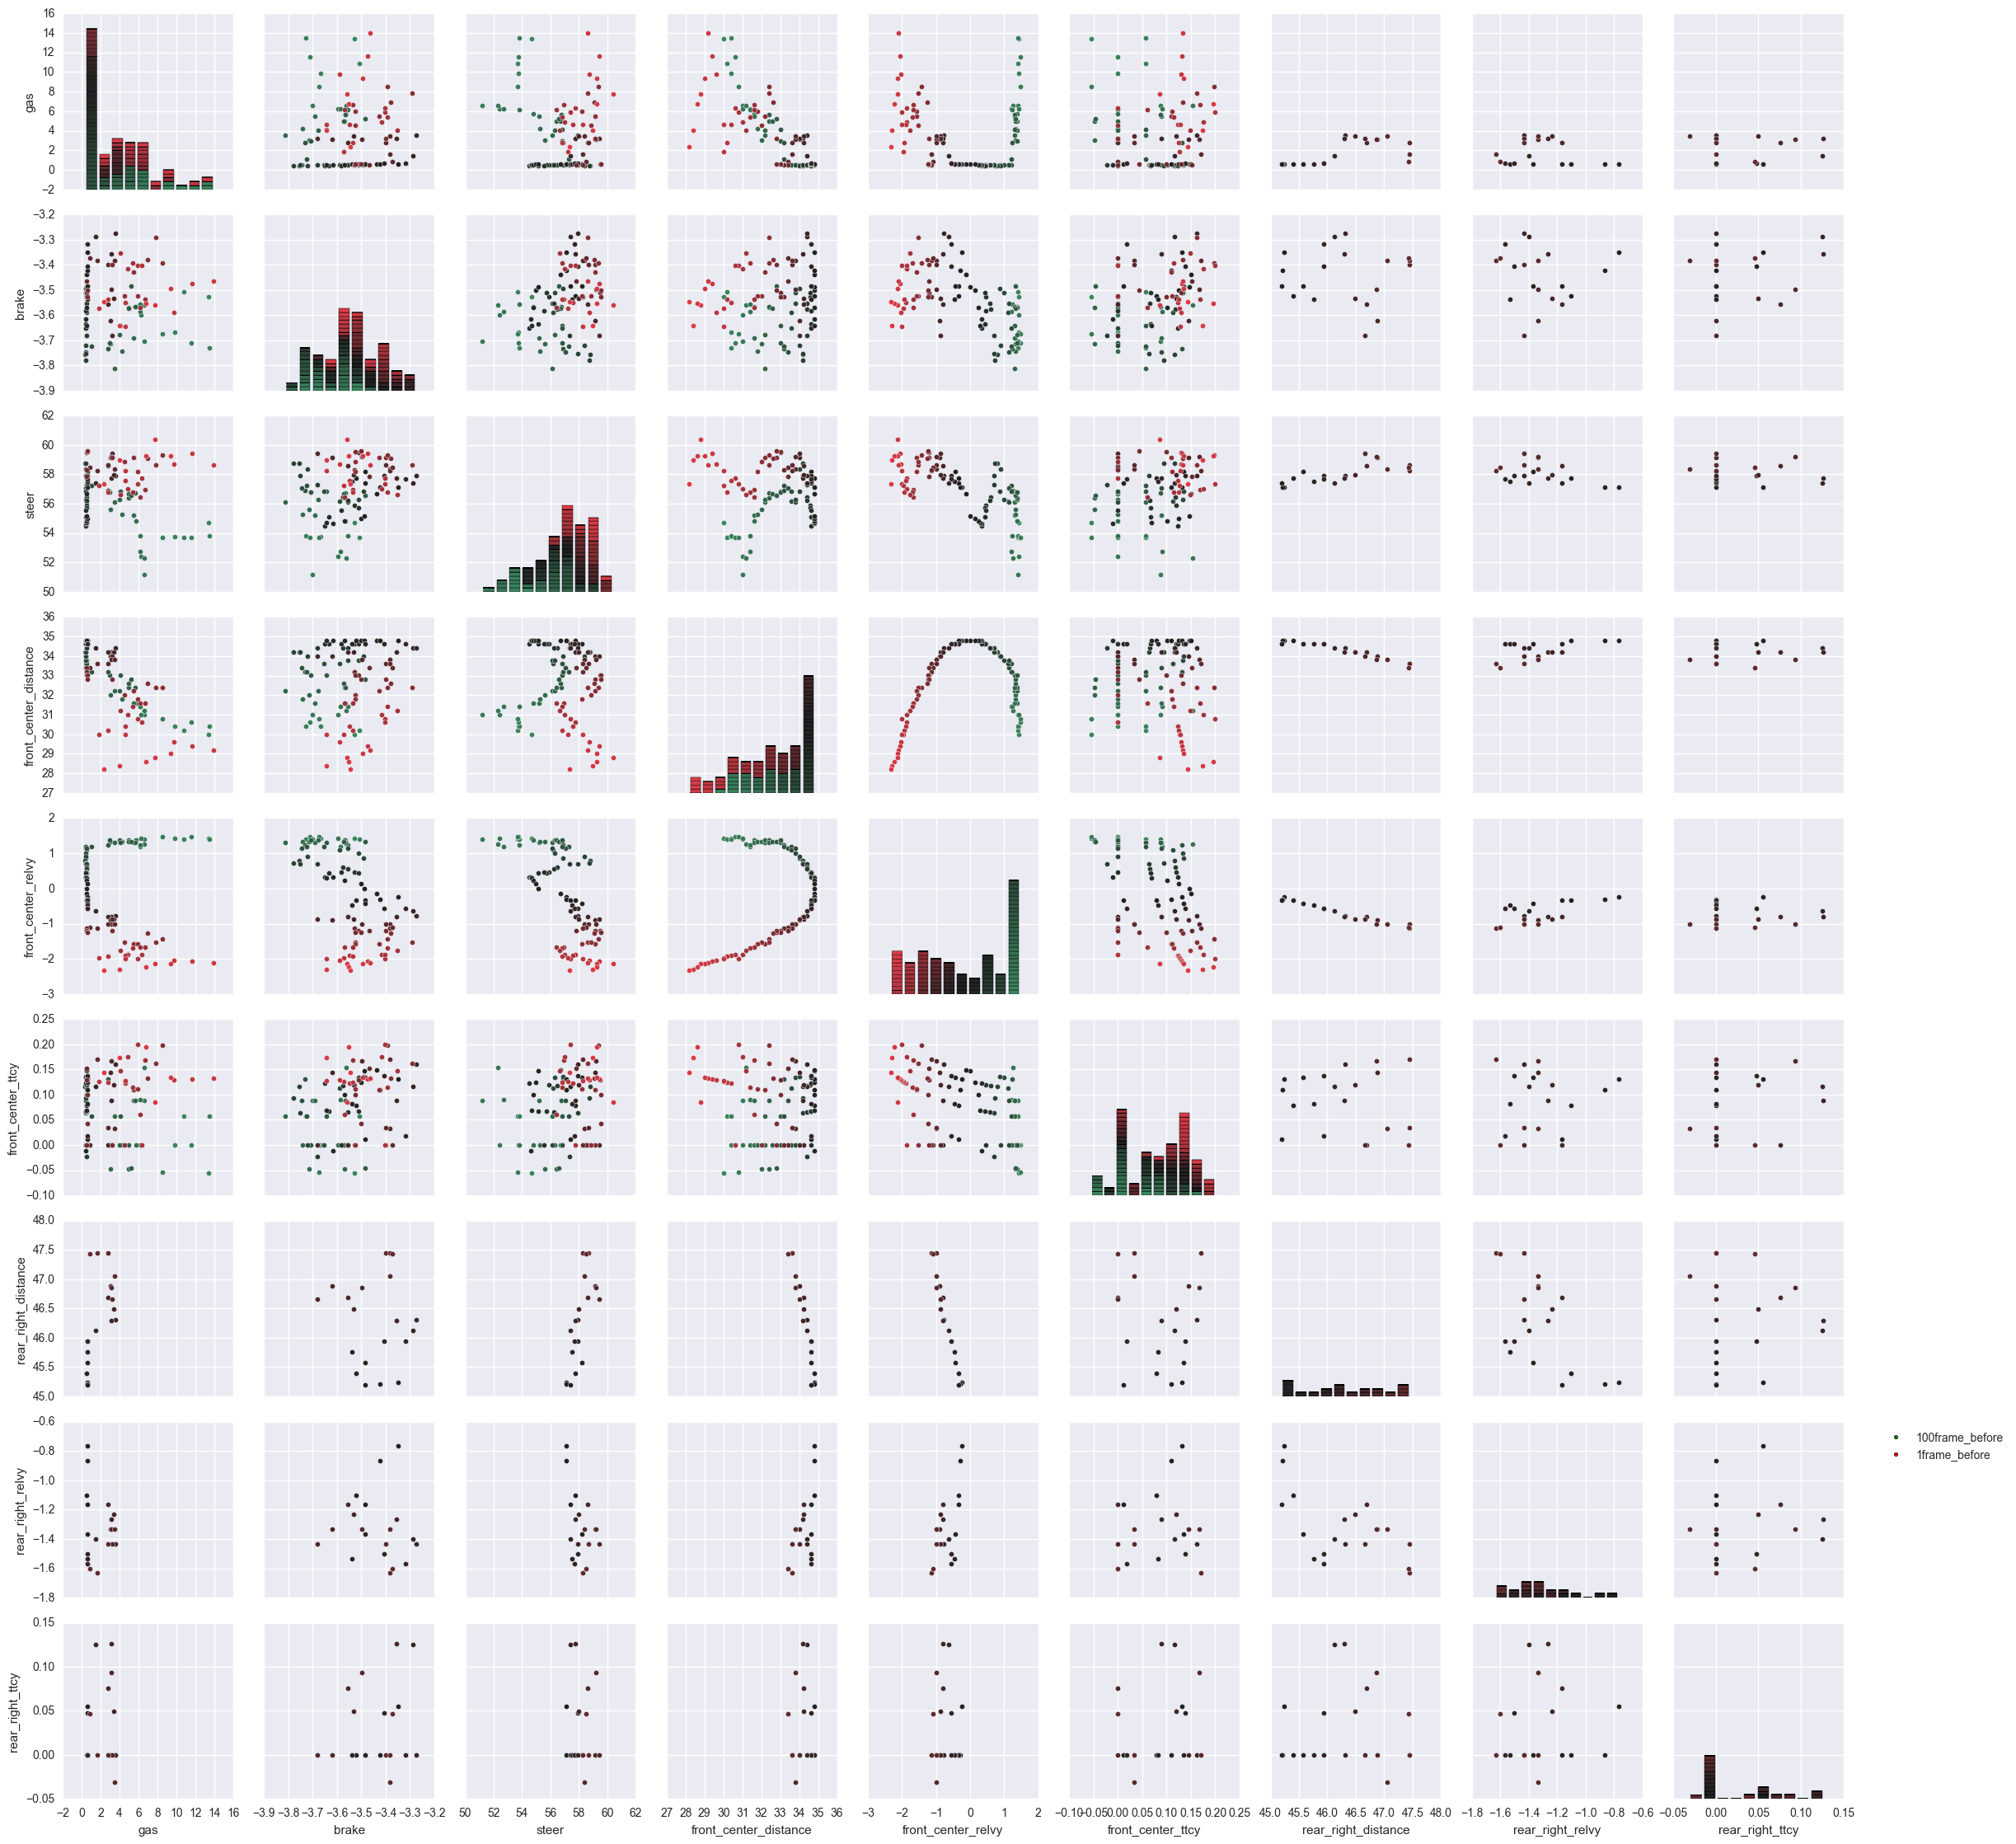
\includegraphics[clip,width=7.0cm]{fig/pairplot_one_lc.png}
    \caption{ある運転行動に対する,車線変更開始10秒前から車線変更開始までの特徴の組み合わせの散布図と,単一の特徴量のヒストグラム.上から(もしくは左から)順番に,アクセル,ブレーキ,ハンドル,前方車両との相対距離,前方車両との相対速度,前方車両との加速度考慮のTTCの逆数,右後方車両との相対距離,右後方車両との相対速度,右後方車両との加速度考慮のTTCの逆数となっている.プロットが緑から赤になるにつれて車線変更開始に近づいていることを示している.}
    \label{fig:pairplot_one_lc}
  \end{center}
\end{figure}
